
\documentclass[tikz,convert={convertexe={magick.exe}}]{standalone}

\begin{document}
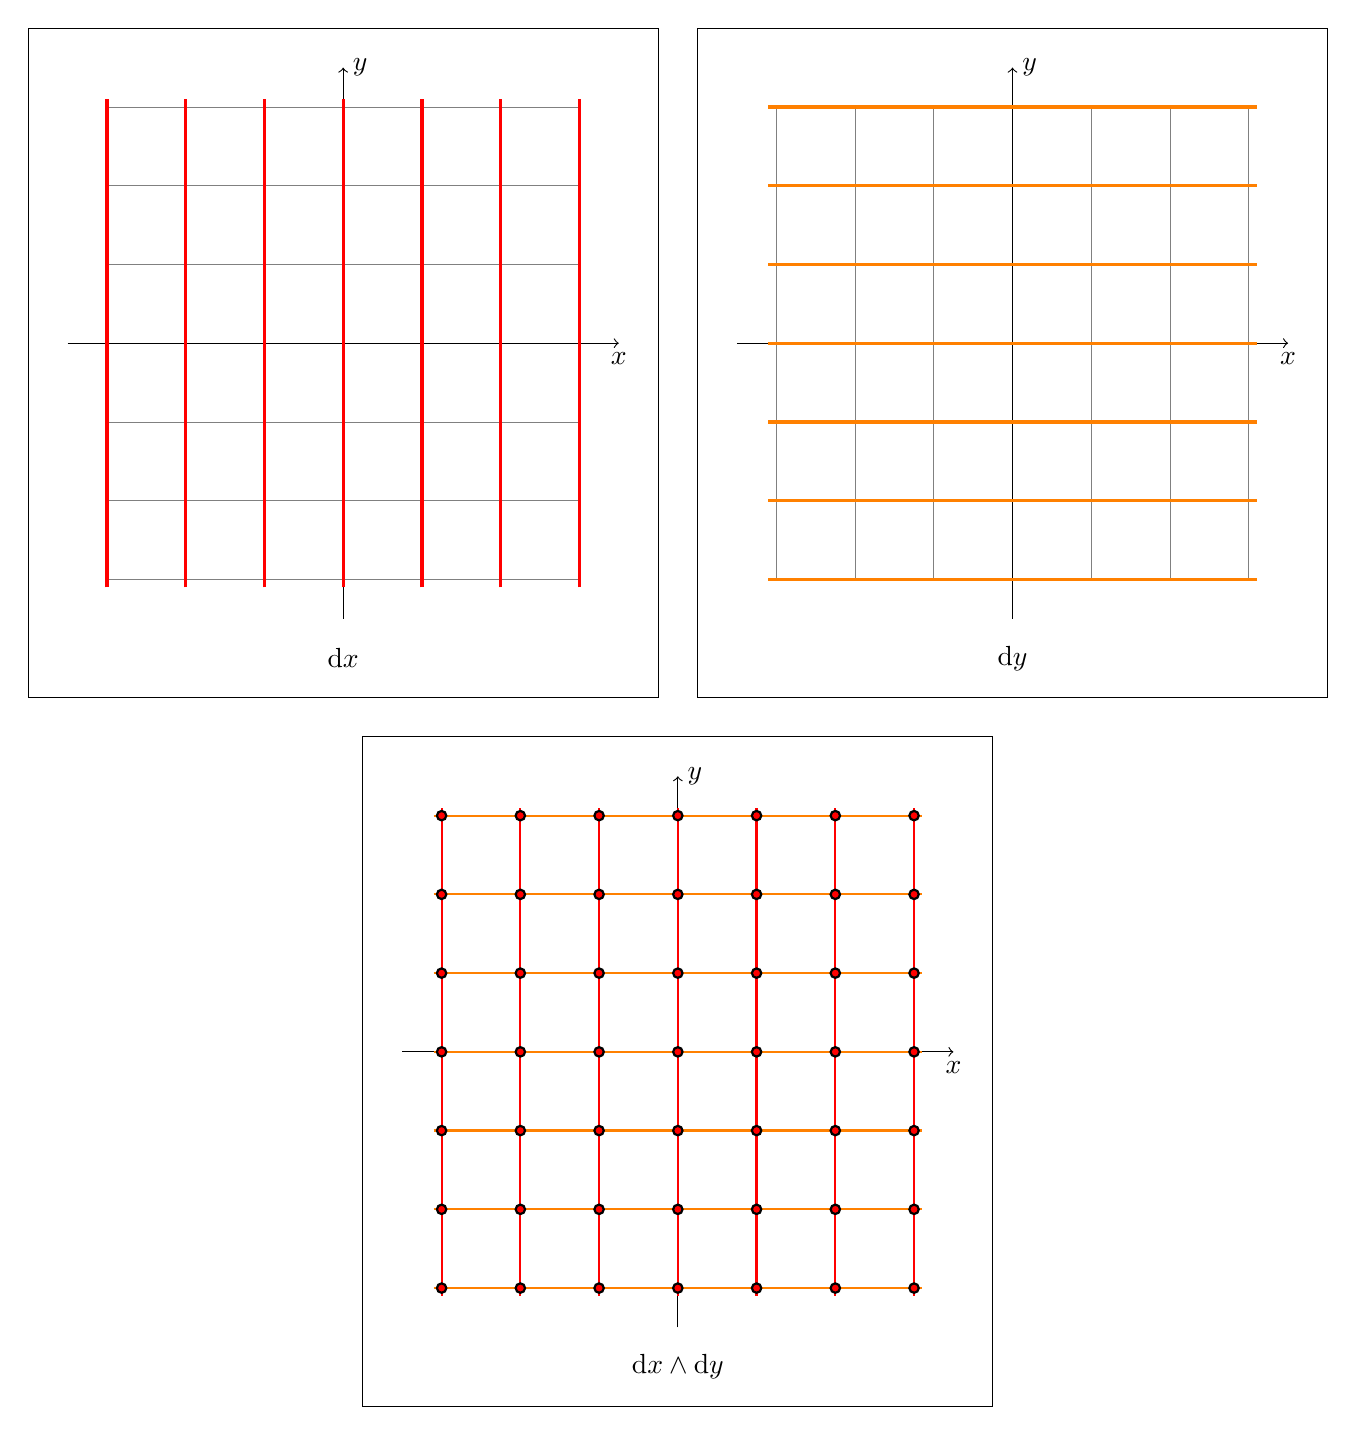
\begin{tikzpicture}

\tikzstyle atom=[circle, draw, inner sep=1.2pt, fill=red, thick]

\begin{scope}
\draw[style=help lines, very thin] (-3,-3) grid (3,3);

\draw[->] (-3.5,0)--(3.5,0) node[below] {$x$};
\draw[->] (0,-3.5)--(0,3.5) node[right] {$y$};

\draw (-4,-4.5) rectangle (4,4);
\node at (0,-4) {$\mathrm{d}x$};

\foreach \x in {-3,-2,...,3}
\draw[very thick,red] (\x,-3.1) -- (\x,3.1);
\end{scope}

\begin{scope}[xshift=8.5cm]\draw[style=help lines, very thin] (-3,-3) grid (3,3);

\draw[->] (-3.5,0)--(3.5,0) node[below] {$x$};
\draw[->] (0,-3.5)--(0,3.5) node[right] {$y$};

\draw (-4,-4.5) rectangle (4,4);
\node at (0,-4) {$\mathrm{d}y$};

\foreach \y in {-3,-2,...,3}
\draw[very thick,orange] (-3.1,\y) -- (3.1,\y);
\end{scope}

\begin{scope}[yshift=-9cm]
\begin{scope}[xshift=4.25cm]
%\draw[style=help lines, very thin] (-3,-3) grid (3,3);

\draw[->] (-3.5,0)--(3.5,0) node[below] {$x$};
\draw[->] (0,-3.5)--(0,3.5) node[right] {$y$};

\draw (-4,-4.5) rectangle (4,4);
\node at (0,-4) {$\mathrm{d}x \wedge \mathrm{d}y$};

\foreach \x in {-3,-2,...,3}
\draw[thick,red] (\x,-3.1) -- (\x,3.1);
\foreach \y in {-3,-2,...,3}
\draw[thick,orange] (-3.1,\y) -- (3.1,\y);

\foreach \x in {-3,-2,...,3}
\foreach \y in {-3,-2,...,3}
\node[atom] at (\x,\y) {};
\end{scope}
\end{scope}
\end{tikzpicture}
\end{document}